\documentclass{article}
\usepackage{iclr2016_conference,times}

\usepackage{float}
\usepackage{hyperref}
\usepackage{url}
\usepackage{amsmath,amssymb}
\usepackage{natbib}
\usepackage{wrapfig}
\usepackage{graphicx}
\usepackage{soul}

\bibliographystyle{abbrvnat}


\usepackage{caption}
\usepackage{subcaption}

\title{
	Mobile Computing (CS23400$/$1) \vspace{-4pt} \\
	{\Large Lab 2 - Report} \vspace{6pt} \\
	{\large Andrea F. Daniele $\hspace{2.2cm}$ Max X. Liu $\hspace{2.2cm}$ Noah A. Hirsch}
}

\begin{document}

\maketitle


\vspace{-1.2cm}

\section{Task}
\vspace{-.3cm}
//TODO

\section{Challenges}
\vspace{-.3cm}
//TODO

\section{Proposed Approach}
\vspace{-.3cm}
//TODO
\begin{wrapfigure}{r}{0.4\textwidth}
    \centering
    \vspace{-18pt}
    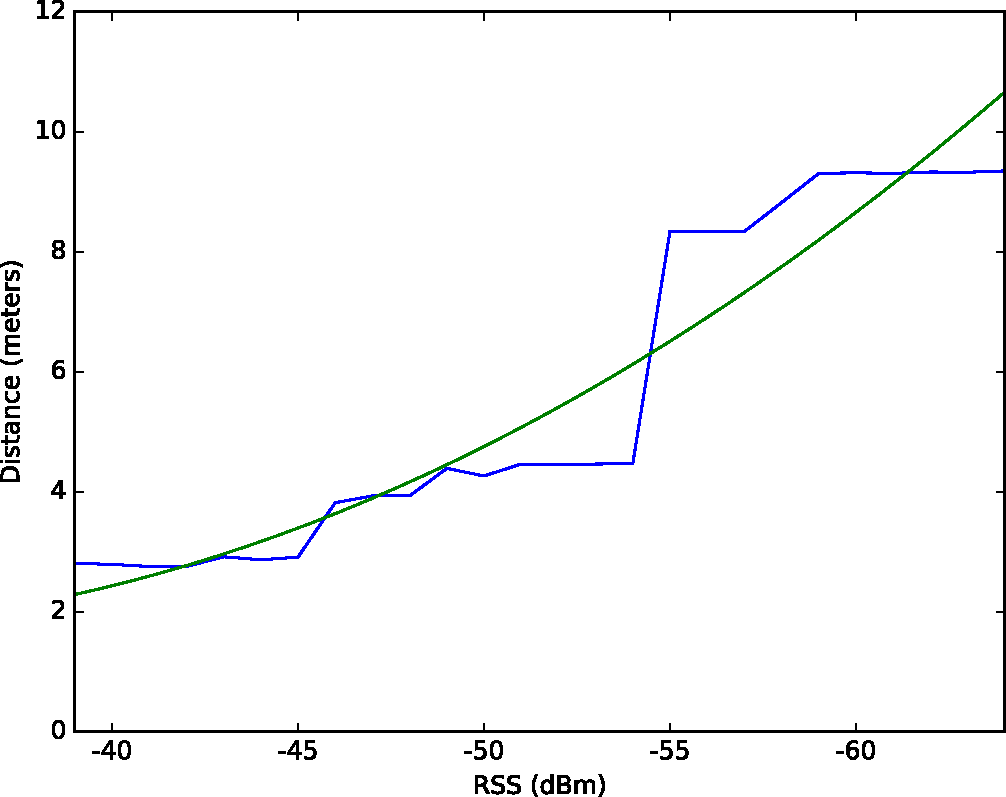
\includegraphics[width=\linewidth]{figures/rss_distance_plot.pdf}
    \caption{RSS-Distance relationship \label{fig:rss_distance_plot}}
\end{wrapfigure}


\section{Results}
\vspace{-.3cm}
We tested out approach on two WiFi camera for which we know the true location. Our
model predicted the location of the two cameras with $XX.XX$ and $XX.XX$ meters error.
Table~\ref{tab:results} shows the predicted location along with the prediction error for the
cameras for which the true location is unknown and the predicted locations for the hidden cameras.

\begin{center}
\begin{table}[h]
\centering
\begin{tabular}{ |c|c|c|c| } 
 \hline
 MAC & Predicted location (meters) & Ground-truth location (meters) & Error (meters) \\ 
 \hline
 8c:85:90:16:0a:a4 & $(7.25, 10.75)$ & $(6.8, 6.8)$ & $3.98$\\ 
 ac:9e:17:7d:31:e8 & $(X.x, Y.y)$ & $(0.87, 9.45)$ & $XX.XX$ \\ 
 d8:c4:6a:50:e3:b1 & $(X.x, Y.y)$ & $-$ & $-$ \\
 f8:cf:c5:97:e0:9e & $(X.x, Y.y)$ & $-$ & $-$ \\
 \hline
\end{tabular}
 \caption{Predicted location and prediction error for four distinct WiFi devices \label{tab:results}}
\end{table}
\end{center}




\section{Conclusion}
\vspace{-.3cm}
//TODO

\bibliographystyle{abbrvnat}
{\scriptsize%
\bibliography{references}
}

\end{document}
